%beamer package
\documentclass[8 pt]{beamer} %nomal size is 8 pt
\usepackage[utf8]{inputenc}
\mode<presentation> %or handout for printing the presentation, but all the poses will be killed with overlaps
{
% As to the theme choices, refer online 
% https://hartwork.org/beamer-theme-matrix/
\usetheme{Berlin}

\usecolortheme{default}
%\usecolortheme{blue}
\useoutertheme{infolines}
\setbeamercovered{invisible} %invisible or transparent
}

\newcommand{\BLUE}{\color[rgb]{0,0,0.69}}
\newcommand{\GREEN}{\color[rgb]{0,0.69,0}}

\title[ACO-OFDM synchronization and channel estimation]{Joint Synchronization and Channel Estimation of ACO-OFDM Systems with Simplified Transceiver}
\author[ L2S ]{  
{\large Xuewen Qian}\inst{1} {\large Honggui Deng}\inst{2} \and {\large Hailang He}\inst{3}
}
\institute[ CentraleSup\'elec ]{
\inst{1}{\large CentraleSup\'elec-CNRS-Universit\'e Paris-Sud, Universit\'e Paris-Saclay}\\
{\large qian.xuewen@l2s.centralesupelec.fr}\\
\medskip
\inst{2} {\large Central South University}
\and
\inst{3} {\large Shaoyang University}
}
\date[15/01/2018]{15/01/2018} %optional
\subject{}
\logo{
\includegraphics[height=0.05\textwidth]{centralesupelec_logo.eps}}
\begin{document}
%\section{Structure}
\begin{frame}
\titlepage
\end{frame}

%\begin{frame}<beamer>{Outline}
%\tableofcontents[currentsection]
%\end{frame}

\AtBeginSection[] { 
  \begin{frame}
    \frametitle{Outline} 
    \tableofcontents[currentsection,hideothersubsections] 
  \end{frame} 
  \addtocounter{framenumber}{-1}  
}

%\section{section}
% a new page
%\AtBeginSection[]
%{
%\begin{frame}{Introduction}
%\tableofcontents[currentsection,currentsubsection] %will emphasis current section
%\end{frame}
%}

\section{Introduction}
\begin{frame}{Introduction}
%\begin{frame}[plain]
%\frametitle{}
%\end{frame}
\begin{block}{Why we need to do research on this?}
\begin{description}
\item[VLC system] Visual light communication (VLC) technology\cite{Chi2015,Qian2016Synchronisation} can provide light and ensure data transmission at the same time.\\
Light emitting diode (LED) \cite{tsonev20143,ferreira2016high} as one of the most popular light sources can promote the widespread utilization of VLC systems.
\item[Drawbacks] 
\begin{enumerate}
\item Multi-path channel
\item Energy efficiency
\end{enumerate}
\end{description}

\end{block}
\pause

\begin{block}{Solution to the drawbacks}
\textbf{\textit{OFDM systems}}$\leftarrow$ Multi-path channel \\
\textbf{\textit{ACO-OFDM systems}}$\leftarrow$ Multi-path channel plus energy efficiency
\end{block}
\pause 

The ACO-OFDM system is the one can solve the two problems \cite{Dissanayake2013Comparison}. 
It is also the core of many modified systems, such as ADO-OFDM, HACO-OFDM and LACO-OFDM \cite{yang2016novel,Wang2017Optical}. In this case, low-complexity transceiver is essential. 
To mitigate the effect of multi-path channels, synchronization and channel estimation are important.

\end{frame}

\section{Low-complexity transceiver}


\begin{frame}
\frametitle{ACO-OFDM systems}
\begin{block}{OFDM system}
Consider an OFDM system with N sub-carriers and the $N_{CP}$ represents CP length. The $X_{i}$ denotes the modulated data on the k-th sub-carrier, then 
\begin{equation}\label{equ:ACO_OFDM_base}
          x(n)=\frac{1}{\sqrt{N}}\sum_{i=0}^{N-1}X_{i}e^{j2\pi\frac{ni}{N}},-N_{CP}\leq n \leq N-1,
\end{equation}
\end{block}
\pause
\begin{block}{Hermitian symmetry}
To make $x(n)$ be real, $X_{i}$ must follow the Hermite symmetry property which is
\begin{equation}\label{equ:Hermite_symmetry}
          X=[X_0,X_1,\ldots,X_{N/2-1},X(N/2),X_{N/2-1}^{*},\ldots,X_{1}^{*}].
\end{equation}
\end{block}

\pause
\begin{block}{ACO-OFDM system}
Only the odd sub-carriers are used and $ x(n)=-x(n+N/2) $ when $
0\leq n\leq N/2-1 $.\\
The $ x(n) $ can be clipped at zero to be $ x_c(n) $ without information loss.
\end{block}

        
\end{frame}

\begin{frame}
\frametitle{VLC channel}
\begin{block}{VLC channel}
\begin{equation}\label{channel_model}
          h(\tau)=\sum_{l=0}^{L-1}g(l)\delta(\tau-\tau_l),
\end{equation}
where $g(l)$ ( $g(l)\geq0$) and $\tau_l$ denote the gain and delay of the l-th transmission path, $\delta(\tau)$ denotes the Dirac function and $L$ represents the number of path.

\end{block}
        
\pause

\begin{block}{Effect of multipath channel on ACO-OFDM signals}
\begin{equation}\label{equ:multipath_effect}
          y(n)=\sum_{l=0}^{L-1}h(l)x_c(n-\tau_l)+w(n),
        \end{equation}
        where $h(l)$ represents the VLC channel time domain response and $w(n)$ denotes the total noise which is modeled as white Gaussian noise\cite{Narmanlioglu2015}.
\end{block}

\end{frame}


\begin{frame}
\frametitle{Low-complexity transmitter}
Denote $ C $ as the first half of $ x(n) $, then $ x=[C;-C] $. If we denote $ A $ and $ B $ as the first half and second half of $ x_c(n) $, then $ C = A - B $. Thus, when $ C $ is generated via IFFT of $ N/2 $ length, $ x(n) $ can be obtained without using IFFT of $ N $ length which reduces the calculation complexity.

%\pause
For $ 0\leq n \leq N/2-1 $, $ C $ can be generated via		
		\begin{eqnarray}\label{equ:sim_transmitter}
			x(n) &=& \sum_{i=0}^{N/2-1} X_{2i+1}e^{j\frac{2\pi}{N}n(2i+1)} \nonumber\\
				 &=& \sum_{k=0}^{N/2-1} X_{k} e^{j\frac{2\pi}{N/2}nk}e^{j\frac{2\pi}{N}n} \nonumber\\
				 &=& IFFT\{X\}_{N/2}e^{j\frac{2\pi}{N}n},
		\end{eqnarray}
		where $ IFFT\{\cdot\}_{N/2} $	represents the IFFT process of $ N/2 $ length.
		
\end{frame}

\begin{frame}
\frametitle{Low-complexity receiver}
Since only the odd sub-carriers are necessary, thus the received data on the $ 2i+1 $ sub-carrier can be obtained as
\begin{eqnarray}\label{equ:sim_receiver}
		%&X_{2i+1}& \nonumber\\
    X_{2i+1}&=& \frac{2}{N}\sum_{n=0}^{N-1} y(n) e^{-j\frac{2\pi}{N}n(2i+1)}\nonumber\\
	&=& \frac{2}{N}\sum_{n=0}^{N/2-1} y(n) e^{-j\frac{2\pi}{N}n(2i+1)}  
	+ \frac{2}{N}\sum_{n=0}^{N/2-1} y(n+N/2) e^{-j\frac{2\pi}{N}(n+N/2)(2i+1)} \nonumber\\
	&=& \frac{2}{N}\sum_{n=0}^{N/2-1} y(n) e^{-j\frac{2\pi}{N}n(2i+1)}  
	- \frac{2}{N}\sum_{n=0}^{N/2-1} y(n+N/2) e^{-j\frac{2\pi}{N}n(2i+1)} \nonumber\\
	&=& \frac{2}{N}\sum_{n=0}^{N/2-1} ( y(n)-y(n+N/2) ) e^{-j\frac{2\pi}{N}n(2i+1)}  \nonumber\\
	&=& \sum_{n=0}^{N/2-1} ( y(n)-y(n+N/2) ) e^{-j\frac{2\pi}{N}n} e^{-j\frac{2\pi}{N/2}ni} \nonumber\\
	&=& FFT\{ ( y(n)-y(n+N/2)) e^{-j\frac{2\pi}{N}n} \}_{N/2},
\end{eqnarray}
where $ FFT\{\cdot\}_{N/2} $	represents the FFT process of $ N/2 $ length.
		
\end{frame}

\section{ZCC pair based scheme}
\subsection{ZCC pair}
\begin{frame}
\frametitle{ZCC pair: two sequences have impulse-like correlation results}
Let $C_p$ and $D_{p+q}$ be the results that $a_n$ and $b_n$ ( $a_n*b_n^*=1$ ) are inverse Fourier transformed into with different order. Then, the two parts can be expressed as
%\begin{columns}[c]
%\column{.45\textwidth}
\begin{equation}
        C_p=\frac{1}{\sqrt{N}}\sum_{n=0}^{N-1} a_n\cdot e^{j2\pi pn/N},
\end{equation}
\begin{equation}
        D_{p+q}=\frac{1}{\sqrt{N}}\sum_{m=0}^{N-1} b_m\cdot e^{j2\pi (p+q)m/N}.
\end{equation}
%\column{.45\textwidth}

We can calculate the periodic correlation between $C$ and $D$ as
    \begin{eqnarray}
         \sum_{p=0}^{N-1} C_p\cdot D_{p+q}^* 
        &=& \frac{1}{N}\sum_{p=0}^{N-1} (\sum_{n=0}^{N-1} a_n\cdot e^{j2\pi pn/N})\cdot (\sum_{m=0}^{N-1} b_m\cdot e^{j2\pi (p+q)m/N})^* \nonumber \\
        %&=& \frac{1}{N}\sum_{p=0}^{N-1} \sum_{n=0}^{N-1} \sum_{m=0}^{N-1} a_n\cdot e^{j2\pi pn/N}\cdot b_m^* e^{-j2\pi (p+q)m/N} \nonumber \\
        &=& \frac{1}{N}\sum_{p=0}^{N-1}\sum_{n=0}^{N-1}\sum_{m=0}^{N-1} a_n\cdot b_m^*\cdot e^{j2\pi p(n-m)/N}\cdot e^{-j2\pi qm/N} \nonumber \\
        &=& \sum_{n=0}^{N-1}\sum_{m=0}^{N-1} a_n\cdot b_m^*\cdot \delta(n-m)\cdot e^{-j2\pi qm/N}
        = \sum_{n=0}^{N-1} e^{-j2\pi qn/N} = N \delta(n)
    \end{eqnarray}
    %where $\delta(n-m)$ denotes the Dirac delta function. Only when $n=m$, $\delta(0)=1$.
%\end{columns}

\end{frame}

\begin{frame}
\frametitle{ZCC pair with PHYDYAS filter}
\begin{columns}[c]
\column{.45\textwidth}
\begin{figure}[htb]
        \centering\includegraphics[width=5cm,height=4.5cm]{the_autocorrelation_of_the_zcc_pair.eps}
        \caption{The non-periodic correlation of the ZCC pair}\label{fig:ZCCauto}
\end{figure}

\column{.55\textwidth}
\begin{figure}[htb]
        \centering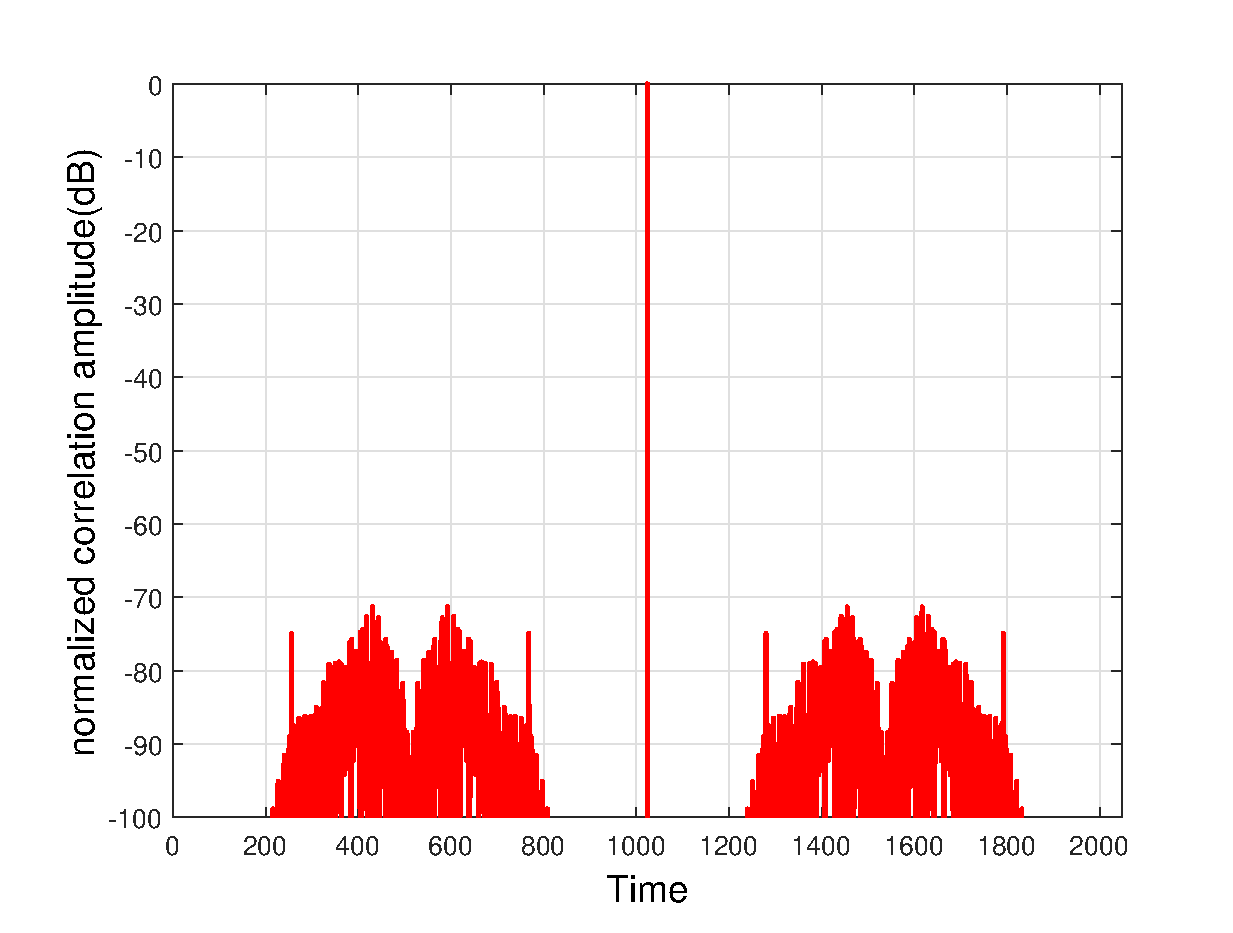
\includegraphics[width=6cm,height=5cm]{PHYDYAS_correlation.eps}
        \caption{ The non-periodic correlation of the ZCC pair with PHYDYAS filter}\label{fig:ZCCauto}
\end{figure}
\end{columns}
By using the PHYDYAS filter, we can approximately ideal impulse-like non-periodic correlation. %This property can be used in synchronization and the calculation

\end{frame}

\begin{frame}
\frametitle{ZCC pair with PHYDYAS filter}
The detailed steps to generate ZCC pair with PHYDYAS filter are listed as:
\begin{description}
\item[Step1] Define $S$ as a vector of $N/16+1$ length consisting of $1$ and $-1$:
        $S=[1, \cdots 1, \cdots -1, \ldots -1]^T$.
\item[Step2] $S$ is multiplied by a matrix $diag([1,j,-1,j^3,\ldots j^{N/16-1},j^{N/16}])$ to be $S_{a}$. This is also called offset quadrature amplitude modulation process.
\item[Step3] Define $S_b$ as a vector with Hermite property via

        $S_b=[S_{a}(0),S_{a}(1),\cdots S_{a}(N/16),S_{a}^*(N/16-1),\cdots S_{a}^*(1)]^T$.
\item[Step4] Inverse Fourier transform the $S_b$ to be $S_c$.
\item[Step5] Finally, we get the required sequence $C$ via $C=[ S_c; S_c; S_c; S_c]\cdot f$. The $fg$ is given in \cite{Bellanger2010}.
\end{description}

\end{frame}

\subsection{Synchronization and channel estimation}
\begin{frame}
\frametitle{Synchronization and channel estimation}
The impulse-like correlation property can be used in synchronization and the calculation results can be used in channel estimation.
\begin{align}\label{equ:gain_acquire}
        %\begin{split}
          %\bar{h}(k)&\nonumber\\
          \bar{h}(k)=&\frac{2}{N}\sum_{n=0}^{N/2-1}(y(n+k)-y(n+k+N/2))D^*(n)\nonumber\\
          =&\frac{2}{N}\sum_{n=0}^{N/2-1}\sum_{l=0}^{L-1}(h(l)(x(n+k-l)-x(n+k-l+N/2))\nonumber\\
          &+w(n+k-l)-w(n+k-l+N/2))D^*(n)\nonumber\\
          =&\frac{2}{N}\sum_{l=0}^{L-1}h(l)\sum_{n=0}^{N/2-1}C(n+k-l)D^*(n)+\tilde{w}(k)\nonumber\\
          =&\sum_{l=0}^{L-1}h(l)\delta(k-l)+\tilde{w}(k).
        %\end{split}
\end{align}
\end{frame}

\begin{frame}
\frametitle{Synchronization and channel estimation}
The preamble in the proposed scheme is $C$. 
The timing offset estimation metric is expressed as
    \begin{eqnarray}\label{equ:synchronization}
          M(k)=\frac{2}{N}\sum_{n=0}^{N/2-1}(y(n+k)-y(n+N/2+k))C^*(n).
    \end{eqnarray}

Then the timing instant is calculated as
    \begin{equation}\label{equ:d}
            \hat k=\arg\max\limits_{k}(\|M(k)\|),
    \end{equation}
    where $\arg\max\limits_{k}(\|M(k)\|)$ means returning the timing instant $\hat k$ when the absolute value of $M(k)$ is the biggest. It performs an one-dimensional search to find $\hat k$.
   
\end{frame}

\begin{frame}
\frametitle{Synchronization and channel estimation}
Since the $ h $ is positive, the negative values in $ \bar{h} $ (obtained from (\ref{equ:synchronization}) ) are set to zero to be $ h^{'} $.

Only the odd sub-carriers are transmitting data. Therefore the simplified channel frequency response is expressed as
    \begin{equation}\label{equ:Channel_Fre_sim}
          H(2k+1)=\sum_{l=0}^{L-1}(h^{'}e^{-j2\pi\frac{\tau_l}{N}})e^{-j2\pi\frac{\tau_l k}{N/2}},0\leq k\leq N/2-1.
    \end{equation}

The received data in frequency domain can be equalized as
    \begin{equation}\label{equ:equalizer}
       X^{'}(2k+1)=\dfrac{2Y(2k+1)}{H(2k+1)},0\leq k\leq N/2-1.
    \end{equation}
   
\end{frame}

\section{Simulation and analysis}
\begin{frame}
\frametitle{Simulation and analysis}
\begin{figure}
        %\setlength{\abovecaptionskip}{-0.1cm}
        %\captionsetup{belowskip=-10pt}
    	\centering 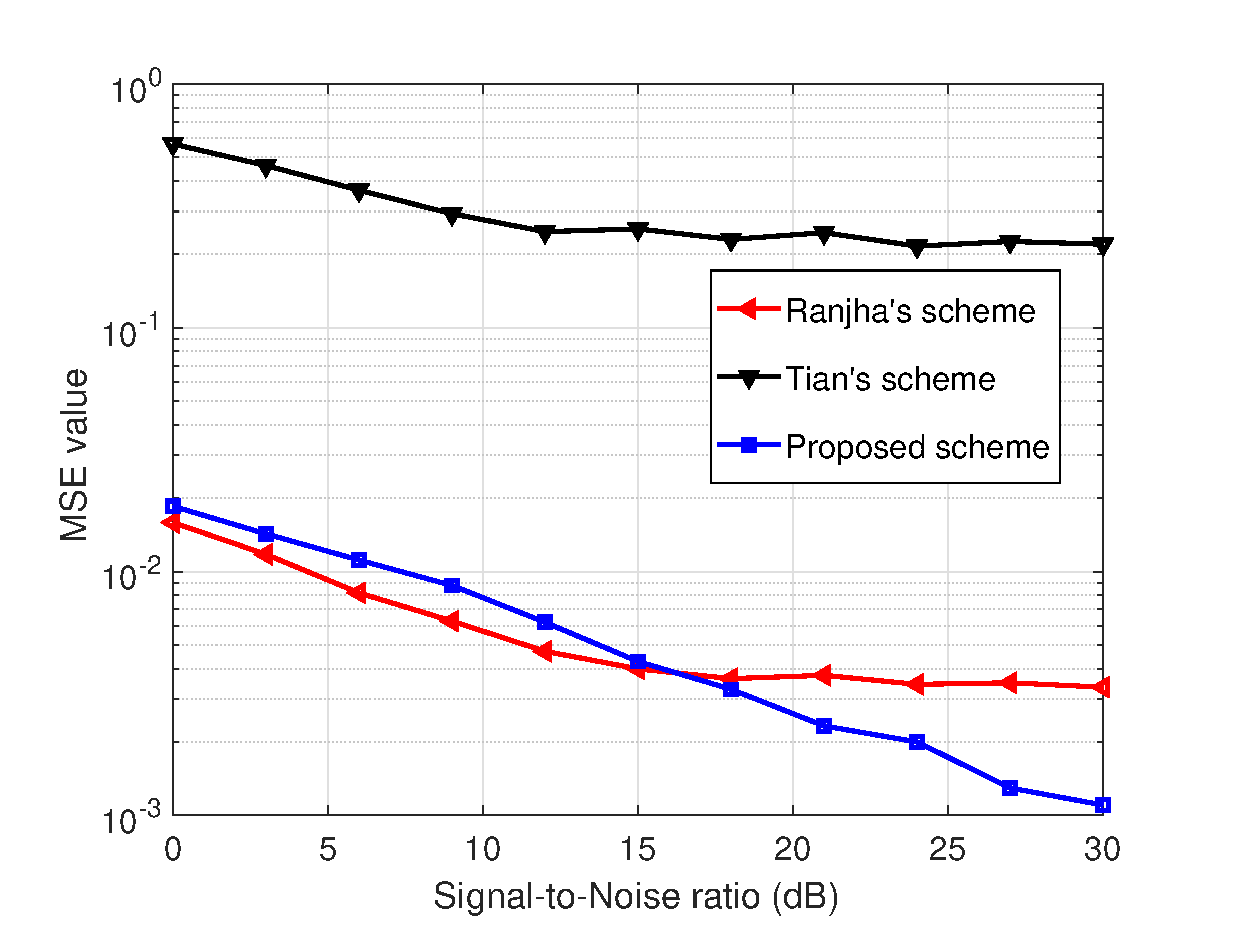
\includegraphics[width=6cm]{synchronization_mse.eps}
		\caption{The MSE performance comparison of synchronization schemes} \label{fig:synchronization_mse}
\end{figure}
 Schemes of \cite{Tian2008} and \cite{Ranjha2015} are selected in performance comparison.
 \begin{itemize}
 \item Good synchronization performance in high SNR region
 \item Tiny performance difference in low SNR region
 \end{itemize}
\end{frame}


\begin{frame}
\frametitle{Simulation}
\begin{columns}[c]
\column{.45\textwidth}
\begin{figure}[!htb]
    	\centering 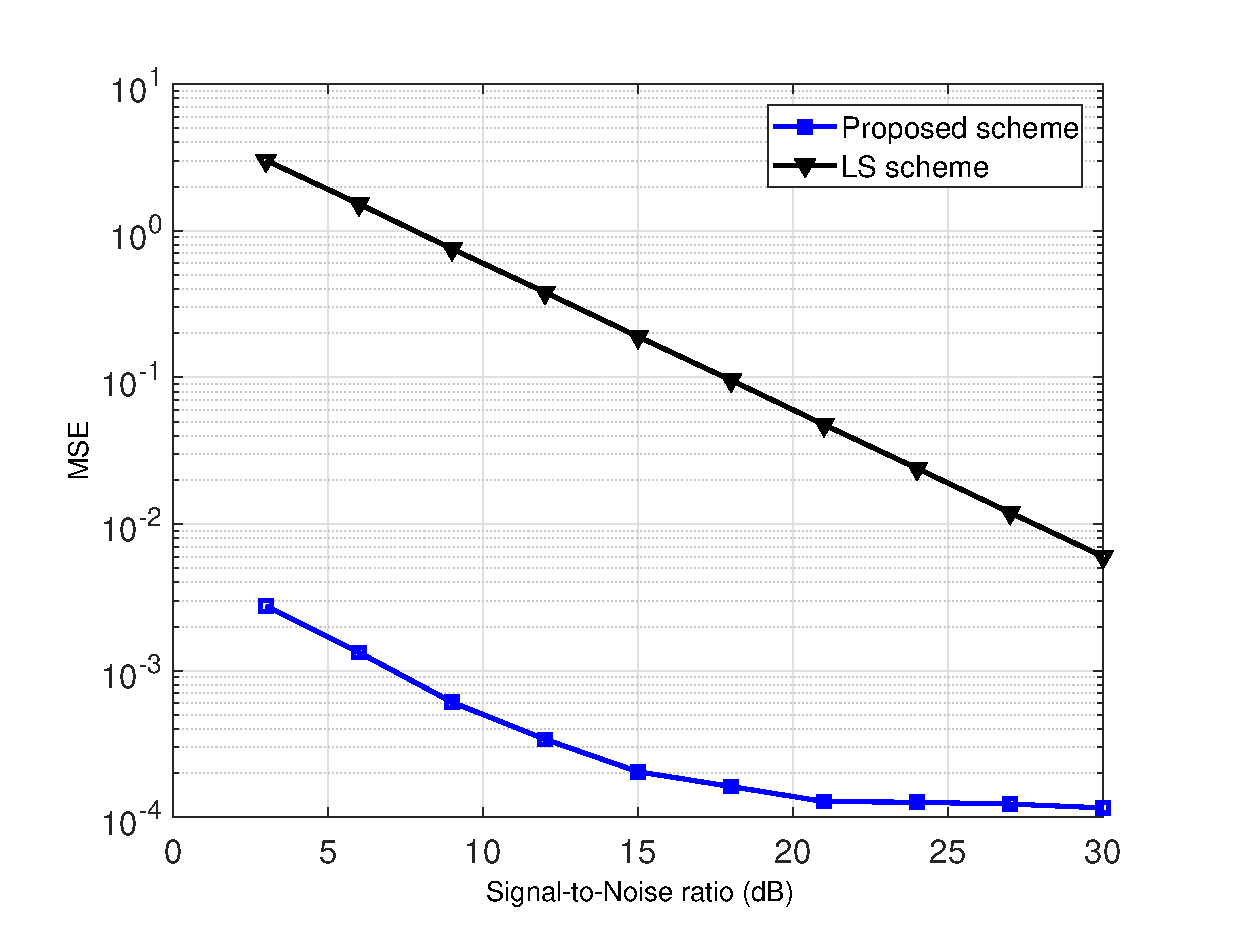
\includegraphics[width=6cm]{channel_estimation_HMSE.eps}
		\caption{The channel frequency estimation performance comparison of LS and proposed scheme}
        \label{fig:channel_estimation_HMSE}
\end{figure}
\column{.45\textwidth}
\begin{figure}[!htb]
    	\centering 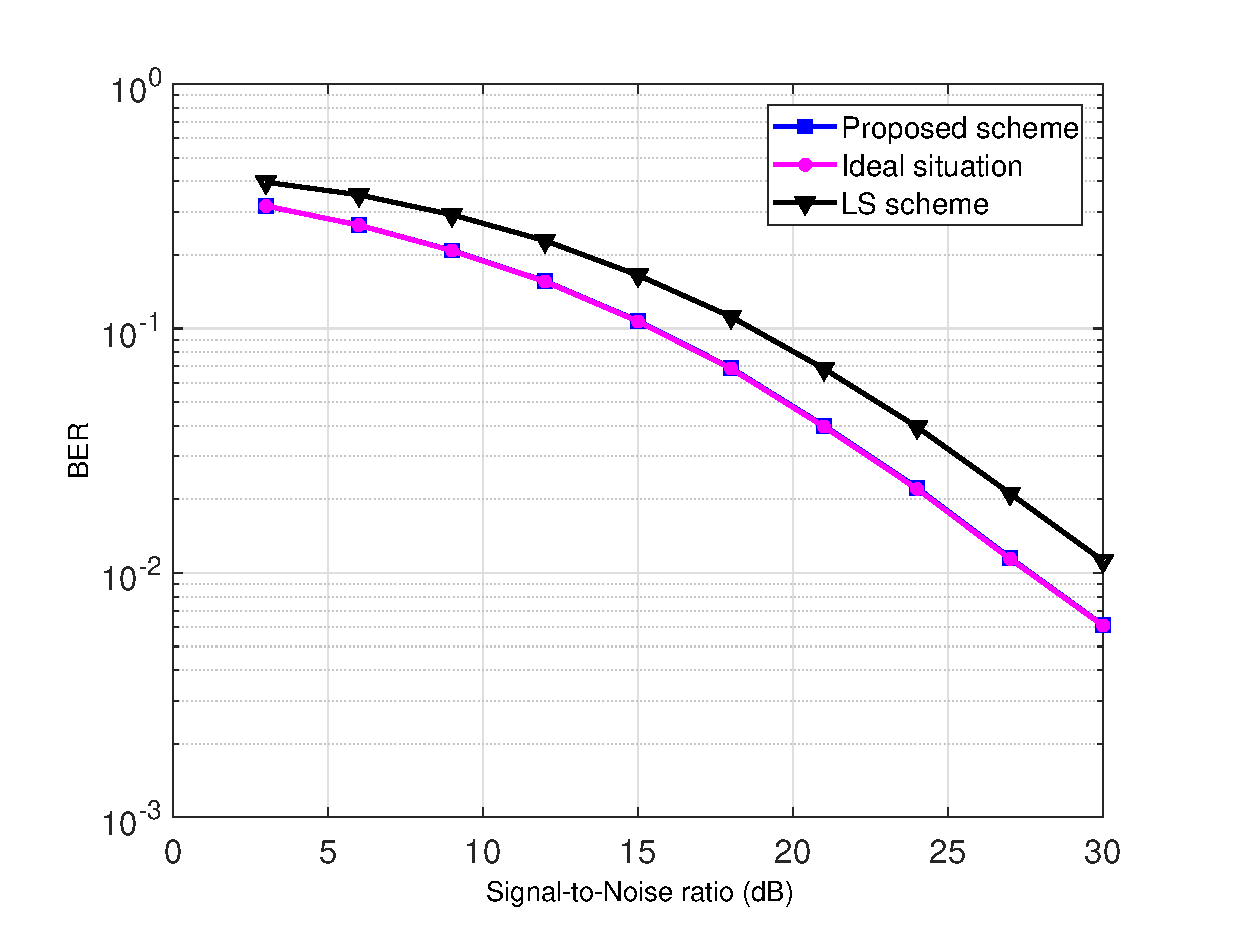
\includegraphics[width=6cm]{channel_estimation_BER.eps}
		\caption{The BER performance comparison of LS and proposed scheme} \label{fig:channel_estimation_BER}
\end{figure}
\end{columns}
\begin{itemize}
\item Good channel frequency response estimation performance 
\item Approximately ideal BER performance
\end{itemize}

\end{frame}


\section{Conclusion}
\begin{frame}
\frametitle{Conclusion}
\begin{block}{}
\begin{itemize}
\item A simplified transceiver is proposed
\item A joint synchronization and channel estimation scheme is proposed
\end{itemize}
\end{block}
\end{frame}

\section*{Acknowledgements}
\begin{frame}
\frametitle{Acknowledgements}
\begin{block}{Support}
This work was supported by Central South University under Post-graduation Innovation Fund project (2016zzts228) and Mittal Innovation Fund project. It is also supported by Research Foundation of Education Bureau of Hunan Province [Project No. 17B238].
\end{block}

\begin{block}{Co-authors}
I'm grateful with the help of Honggui Deng from Central South University and Hailang He from Shaoyang University.
\end{block}

\end{frame}

\begin{frame}
\centerline{ {\Huge Thank you !}  }
\begin{figure}
    	\centering 
\includegraphics[width=6cm]{centralesupelec_logo.eps}
		%\caption{The MSE performance comparison of synchronization schemes} \label{fig:synchronization_mse}
\end{figure}
\end{frame}

\begin{frame}[allowframebreaks]{References} 
\bibliographystyle{apalike}
\bibliography{mybibtex}
\end{frame}




\end{document}


%used for blocks inside slide:
%\only{1,3} %it won't be shown in page 1 and 3 %mind the moving of blocks two fill the gaps between
%\uncover{1,3} %it will be shown in page 1 and 3 %it will leave the space of blocks